\chapter{Algorithmen zur Erkennung von SLTR}

Im vorherigen Kapitel wurden Kriterien für die Existenz einer SLTR erarbeitet, die allerdings nicht sofort einen Algorithmus, sowohl zur Frage nach der Existenz, als auch zum erlangen einer spezifischen SLTR liefern. Diesem Thema wollen wir uns nun im folgenden Kapitel zuwenden und dafür zum Einstieg einen von Aerts und Felsner in \cite{af13} erarbeiteten Algorithmus betrachten.

\section{SLTR via Zwei-Fluss}

Wir betrachten im folgenden gerichtete Graphen. Das Ziel ist es, für einen gegebenen Graphen sowohl einen Schnyder Wood als auch ein FAA jeweils als Lösung eines Fluss-Problems zu erhalten und diese beiden dann in einem Zwei-Fluss-Problem zu kombinieren, sodass eine Lösung ein Ecken-Kompatibles-Paar gibt und wir somit eine SLTR erhalten. Wir beschäftigen uns also mit der folgenden Problemstellung.

\begin{definition}[Gerichtetes-Multi-Fluss-Problem]
Sei $D=(V,E)$ ein gerichteter Graph, im Weiteren auch Netzwerk genannt, mit den Kapaziäten $c:E\mapsto\mathbb{R}_{+}$, Paaren von ausgezeichneten Knoten $\{(s_1,t_1), ... ,(s_n,t_n)\}$ und positiven Bedarfen $\{d_1, ... ,d_n\}$, dann ist $\varphi=(\varphi_1, ... ,\varphi_n)$ ein zulässiger Fluss, falls
\begin{itemize}
\item[F1] $\forall (u,v) \in E : \sum_{i=1}^{n}{\varphi_i(u,v)} \leq c(u,v) $
\item[F2] $ \forall u \neq s_i,t_i : \sum_{w \in V} \varphi_i(u,w) - \sum_{w \in V} \varphi_i(w,u) $
\item[F3] $ \forall s_i : \sum_{w \in V} \varphi_i(s_i,w) - \sum_{w \in V} \varphi_i(w,s_i) = d_i $
\item[F4] $ \forall t_i : \sum_{w \in V} \varphi_i(w,s_i) - \sum_{w \in V} \varphi_i(s_i,w) = d_i $
\end{itemize}
\end{definition}

Im Fall $n=1$ und Kapazitäten $c:E\mapsto\mathbb{N}$ impliziert die Existenz eines zulässigen Flusses die Existenz einer ganzzahligen Lösung. Für $n=2$ und wir ungerichtete Netzwerke zeigt \cite{hu} die selbe Eigenschaft. Dies gilt jedoch im Fall $n \geq 2$ für gerichtete Graphen nicht mehr.\\

\subsection{Schnyder-Wood-Fluss}

Um einen Schnyder Wood als Fluss-Problem zu kodieren, kann man die in Abschnitt \ref{alpha_orientations} eingeführten $\alpha_s$-Orientierungen auf dem Abschluss von $G+G^*$ nutzen. Fusy zeigt in \cite{fusy07} im Zuge der Untersuchung spezifischer $\alpha$-Funktionen, dass sich $\alpha_s$-Orientierungen von $G+G^*$ in linearer Zeit berechnen lassen, sodass wir auch einen Schnyder Wood auf $G$ in linearer Zeit erhalten.\\

Machen wir uns also an die Konstruktion eines Netzwerks $\mathcal{N}_S$ mit einer Quelle und Senke, sodass eine zulässige Lösung $\varphi_S$ einer $\alpha_s-Orientierung$ von $\tilde{G}$ entspricht, und somit auch einen Schnyder Wald auf $G$ liefert. Besonderes Augenmerk ist hier auf die Möglichkeit einer späteren Kombination mit einem FAA Fluss gelegt, um ein Kombiniertes Netzwerk zu erstellen, und nicht unbedingt auf Effizienz.\

Wie oben schon erwähnt ist $\tilde{G}$ bipartit, Kanten-Knoten haben Grad 4, Knoten-Knoten Grad $deg(v)$ und Gebiets-Knoten Grad $|f|$. Für eine $\alpha_s$-Orientierung muss jeder Kanten-Knoten Ausgrad 1, jeder Knoten-Knoten Eingrad $deg(v)-3$ und jeder Gebiets-Knoten Eingrad $|f|-3$ haben. Die Kanten-Knoten am äusseren Gebiet sind in $\tilde{G}$ immer nach aussen orientiert. Somit müssen wir nur die inneren Kanten-Kanten $E_{in}$ betrachten. \

\begin{figure}[h]
	\centering
  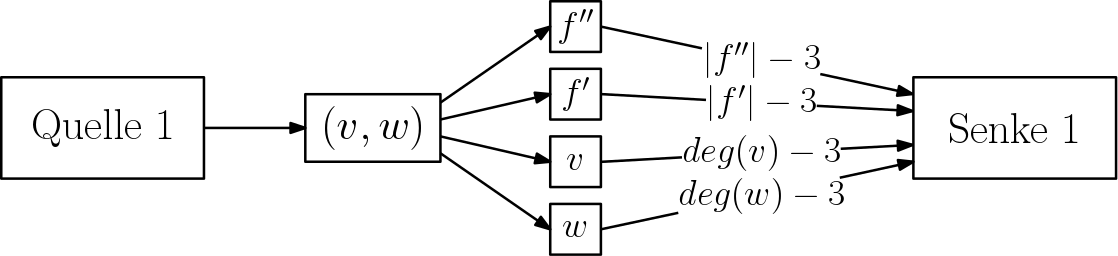
\includegraphics[width=0.9\textwidth]{schnyder_flow.png}
  \caption{Der Schnyder Wood Fluss durch eine innere Kante $(v,w)$.}
  \label{schnyder_flow}
\end{figure}

Sei $\mathcal{N}_S$ ein Netzwerk mit jeweils einer Quelle $s$ und Senke $t$, Kanten von der Quelle zu jedem $e \in E_{in}$ mit Kapazität 1, Kanten von den Kanten-Knoten $e$ zu inzidenten Knoten-Knoten $v$ und (inneren) Gebiets-Knoten $f \in F_{in}$ in $G$ ebenfalls mit Kapazität 1, Kanten von $f \in F_{in}$ zur Senke mit Kapazitäten $|f|-3$, Kanten von den (inneren) Knoten-Knoten $v \in V_{in} = V \setminus \{a_1,a_2,a_3\}$ zur Senke mit Kapazitäten $deg(v)-3$ und Kanten von den Aufhängungen $a_i$ zur Senke mit Kapazitäten $deg(a_i)-2$. Die letzte Kapazität resultiert aus dem Fakt, dass die Halbkante in $G+G^*$ von $a_i$ aus immer nach aussen orientiert ist und wir somit nur noch zwei andere Kanten nach aussen orientieren müssen.

Der Bedarf des Netzwerkes entspricht der Anzahl der inneren Kanten von $G$. Sei nun $\varphi_S$ eine zulässige ganzzahlige Lösung, dann hat jeder Kanten-Knoten $e$ Ausgrad 1. Der Fluss $\varphi_S$ entlang einer Auskante von $e \in E_{in}$ in $\mathcal{N}_S$ entspricht dann genau der hin zu $e$ orientierten Kante einer $\alpha_{s}$-Orientierung auf $G+G^*$. Die Knoten-Knoten und Gebiets-Knoten haben $deg(v)-3$ bzw. $|f|-3$ von $\varphi_S$ genutzte Auskanten und somit entspricht hier eine leere Kante in $\mathcal{N}_S$ einer von $v$ bzw. $f$ weg orientierten Kante bezüglich $\alpha_{s}$. Ein zulässiger ganzzahliger Fluss $\varphi_S$ kodiert also eine $\alpha_s$-Orientierung auf $G+G^*$. Somit existiert genau dann ein Schnyder Wald auf $G$, wenn eine ganzzahlige Lösung $\varphi_S$ für $\mathcal{N}_S$ existiert.

\subsection{FAA-Fluss}\label{faa-flow}

Um ein FAA für einen planaren Graphen $G$ zu erhalten, müssen wir jedem Gebiet $f \in F$ genau drei Ecken und $|f|-3$ flache Winkel zuordnen und jeder Knoten darf maximal einem Gebiet zugeordnet werden, also in diesem flach sein. Falls eine Einbettung und die Aufhängungen $\{a_1,a_2,a_3\}$ gegeben sind, müssen wir jedem inneren Gebiet $f \in F_{in}$ drei Ecken und $|f|-3$ flache Winkel zuweisen und jeder innere Knoten $v \in V_{in}$ darf maximal einem Gebiet zugeordnet werden. Wir konstruieren ein Netzwerk für den zweiten Fall, das sich leicht verallgemeinern lässt.\

Sei also wieder $\mathcal{N}_F$ ein Netzwerk mit einer Quelle und Senke, einem Knoten für jeden inneren Winkel $(f,v)$, mit $v\in V$ und $f \in F_{in}$, Knoten für alle inneren Gebiete $f$ und alle inneren Knoten $v$. Von der Quelle existiert eine Kante mit Kapazität 1 zu jedem inneren Winkel $(f,v)$, von jedem inneren Winkel $(f,v)$ jeweils eine Kante zu $f$ und zu $v$ mit Kapazität 1, von jedem inneren Gebiet $f$ eine Kante mit Kapazität 3 zur Senke und zuletzt noch eine Kante von jedem inneren Knoten $v$ zur Senke mit Kapazität 1. Der Bedarf des Netzwerks ist $\sum_{f \in F_{in}}{|f|}$ und entspricht der Anzahl der inneren Winkel von $G$. 

\begin{figure}[h]
	\centering
  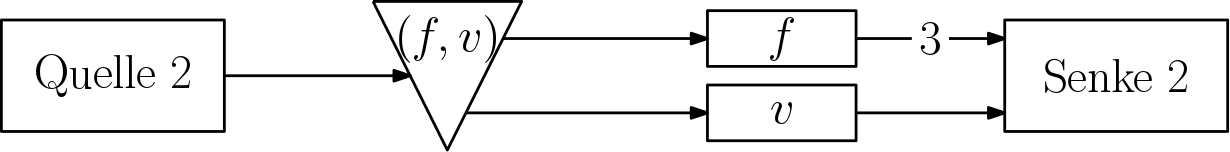
\includegraphics[width=0.8\textwidth]{faa_flow.png}
  \caption{Der FAA-Fluss durch einen Winkel $(f,v)$.}
  \label{faa_flow}
\end{figure}


Sei $\varphi_F$ ein zulässiger ganzzahliger Fluss, dann entspricht Fluss auf einer Kante $((f,v),f)$ einer Ecke (eines möglichen GFAAs) von $f$ und Fluss auf $((f,v),u)$ der Zuweisung eines Knoten zu $f$, also einem flachen Winkel in einem GFAA. Zur Vereinfachung sprechen wir im Weitern auch von Ecken- respektive Zuweisungs-Fluss. Somit wird jeder innere Winkel entweder dem Gebiet zugewiesen oder als Ecke ausgezeichnet und es kann nur jeweils ein Winkel an jedem inneren Knoten zugewiesen werden. $\varphi_F$ respektiert also die Bedingungen aus Definition \ref{def_faa} und es existieren nur dann FAAs auf $G$, wenn mindestens eine ganzzahlige Lösung für $\mathcal{N}_F$ existiert. Eine spezifische Lösung $\varphi_F$ entspricht genau einem FAA auf $G$.

\begin{remark}

Das oben konstruierte Netzwerk zur Bestimmung von FAAs lässt sich auch als Zwei-Fluss Problem konstruieren, wenn wir für Ecken- und Zuweisungs-Fluss getrennte Quellen und Senken einführen. Der Bedarf des Ecken-Flusses ist dann $3|F_{in}|$ und der Bedarf des Zuweisung-Flusses $\sum_{f \in F_{in}}{|f|-3}$.

\begin{figure}[h]
	\centering
  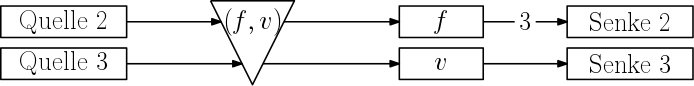
\includegraphics[width=0.8\textwidth]{faa_2_flow.png}
\end{figure}

Eine zulässige ganzzahlige Lösung $\varphi_F = (\varphi_{F_2},\varphi_{F_3})$ entspricht dann wieder einem FAA auf $G$, da aus der Ganzzahligkeit folgt, dass ein Winkel entweder von $\varphi_{F_2}$ oder $\varphi_{F_3}$ genutzt wird und somit eine Definition \ref{def_faa} respektierende Beschriftung der Winkel vorliegt.

\end{remark}




%% Graphs with exponentially many Schnyder Woods and/or FAAs exist....

\subsection{Das Zwei-Fluss Netzwerk}

Nachdem wir nun sowohl für Schnyder Woods als auch für FAAs ein Netzwerk betrachtet haben, für das eine ganzzahlige Lösung eine einen Schnyder Wood bzw. ein FAA auf $G$ liefert, wollen wir jetzt eine Kombination aus beiden erstellen...

